\chapter{研究方法}


在智能交通里,多目标跟踪技术特别关键,它是交通流量监测、智能驾驶辅助和交通事件预警等功能的核心技术之一。本文主要就是想优化现有的多目标跟踪模型,然后在仿真场景里测试一番,来提升跟踪算法的性能和可靠性。


\section{数据收集与预处理}



\subsection{基于仿真场景Town10的交通场景视频收集}


我为了收集高质量的训练和测试数据,选择在CARLA仿真平台的Town10场景里开展数据收集工作。如图\ref{fig:p5}所示,Town10场景是一个复杂的城市交通环境,涵盖多种道路类型、交通标志、信号灯,还有车辆和行人等动态交通参与者。通过在该场景下运行仿真脚本,我们能够生成高清交通场景视频,同时记录下目标的真实轨迹(Ground Truth)。


\begin{figure}[htbp] % 可以是h(here),t(top),b(bottom),p(page of floats)
	\centering
	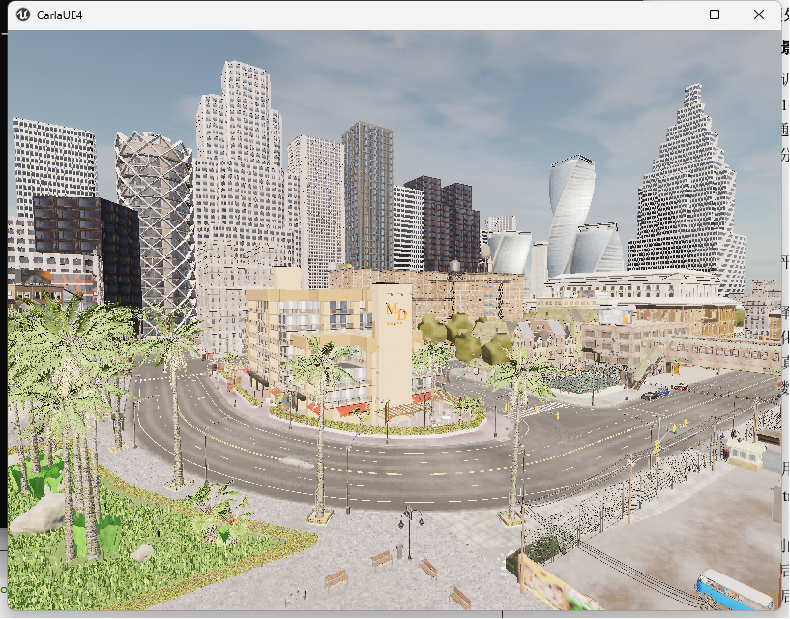
\includegraphics[width=1\textwidth]{p5} % 假设图片文件名为car.pdf或car.png等,位于当前工作目录
	\caption{仿真场景Town10} % 图片标题
	\label{fig:p5} % 用于引用的标签
\end{figure}





\subsubsection{仿真环境搭建}

安装CARLA仿真平台:使用CARLA 0.9.15版本,确保其支持多传感器数据输出和高精度的交通模拟。

配置仿真场景:选择Town10场景,并设置不同的天气条件、时间段和交通流量,以模拟真实世界中的多样化交通场景。

传感器配置:在仿真车辆上安装多个传感器,包括RGB摄像头、激光雷达和毫米波雷达,以获取多模态数据。

\subsubsection{视频数据收集}

运行仿真脚本:使用Python脚本控制仿真车辆的行驶路径,同时记录摄像头的视频流。本项目中使用了traffic twin项目中的 Drive.py文件,通过调整参数选择不同的控制器和传感器配置。

数据存储:将收集到的视频数据存储为序列化的文件格式。本项目中,我们在Town10场景中运行500秒,然后将每一帧截取下来,每一帧都是一张图片。最终将它们保存在同一个文件夹中,用于后续处理。



\subsection{从模拟器中获取Ground Truth数据}

为了评估跟踪算法的性能,得先获取目标的真实轨迹作为Ground Truth。CARLA仿真平台它能提供目标的详细信息,像位置、速度、方向这些关键数据都很精准。


\subsubsection{Ground Truth数据提取}

传感器数据同步:在仿真过程中,同步记录传感器数据和目标的真实状态信息。通过CARLA的API,可以获取每个目标在每一帧中的精确位置、速度和方向,如图\ref{fig:p29}

数据格式化:将Ground Truth数据格式化为结构化的文件格式,以便与视频数据进行匹配和分析。





\begin{figure}[htbp] % 可以是h(here),t(top),b(bottom),p(page of floats)
	\centering
	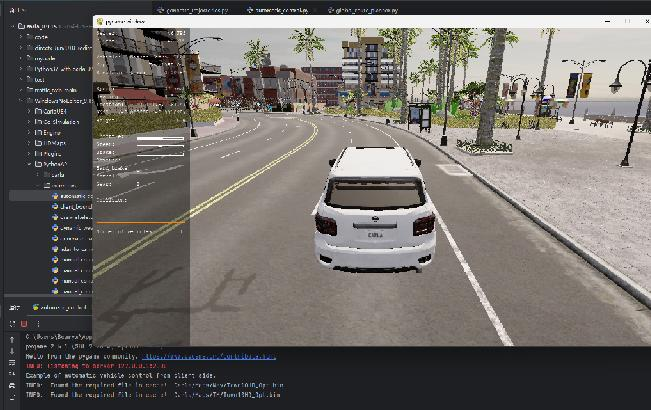
\includegraphics[width=1\textwidth]{p29} % 假设图片文件名为car.pdf或car.png等,位于当前工作目录
	\caption{数据提取} % 图片标题
	\label{fig:p29} % 用于引用的标签
\end{figure}



\subsubsection{数据预处理}

数据清洗:去除噪声数据和异常值,确保数据的准确性和一致性。

数据标注:对视频数据进行标注,标记每个目标的类别(如车辆、行人)和边界框位置。可以使用自动化标注工具或人工标注方法。

数据增强:通过数据增强技术(如旋转、缩放、裁剪)扩充数据集,提高模型的泛化能力。

\section{模型设计与优化}



\subsection{现有检测跟踪模型的分析}


在智慧交通里,多目标跟踪主要是做两件事:目标检测和数据关联。现在常用的模型有两类,一类是基于检测的跟踪(Track-by-Detection),另一类是端到端跟踪(End-to-End Tracking)。基于检测的跟踪通俗来讲,就是先用目标检测算法在每一帧图像里把潜在目标给挑出来,然后再用数据关联算法,把这些目标候选和已有的轨迹匹配起来,就像先找人,再跟踪他们的动作一样。而端到端跟踪就更深奥了,它用深度学习直接把目标检测和数据关联整合到一个模型里,图像序列一输进去,目标的运动轨迹就直接出来了。


\subsubsection{基于检测的跟踪模型}

为确定目标位置,常用 YOLO、Faster R-CNN 和 SSD 等检测算法,它们在速度与准确性上有不同表现。就像 YOLO 算法,速度飞快,能实时给出结果,不过准确性稍逊一筹;而 Faster R-CNN 则更注重准确性,检测结果细致入微,但计算过程复杂,速度上稍慢。


\subsubsection{端到端的跟踪模型}


深度学习模型构建时,端到端跟踪架构经常把卷积神经网络(CNN)和循环神经网络(RNN)结合起来。就说经典算法吧,SORT 算法把卡尔曼滤波和匈牙利算法结合起来,搭建起一个高效的在线实时跟踪框架。DeepSORT 算法更厉害,它在 SORT 的基础上,加入深度学习特征提取模块,利用外观特征建模,增强跟踪在复杂场景下的稳定性。

不过,端到端跟踪模型的复杂度相对较高,训练时需要大量计算资源和大规模标注数据集来支撑它的训练过程。但智慧交通对实时性要求很高,所以在实际应用中就得对模型进行优化设计。常见的优化方法有引入轻量级网络架构,降低计算负载;或者通过模型压缩技术,像剪枝、量化之类的,来提升推理效率。这样,模型在保持性能的同时也能满足实时性的要求。
\subsection{模型优化策略与方法}

\subsubsection{模型结构优化}

轻量级网络设计:采用轻量级的卷积神经网络(如MobileNet、ShuffleNet)作为目标检测模块,减少计算复杂度,提高实时性。

特征融合:结合多模态数据(如RGB图像、激光雷达点云)进行特征融合,提高目标检测和跟踪的准确性。可以使用注意力机制和多尺度特征融合技术,增强模型对复杂场景的适应能力。

模型压缩与加速:通过剪枝、量化和知识蒸馏等技术,对预训练模型进行压缩和加速,降低模型的存储和计算需求。

\subsubsection{数据关联优化}

改进关联算法:引入深度学习特征提取,如使用ResNet或Inception网络提取目标的外观特征,结合卡尔曼滤波和匈牙利算法进行数据关联,提高关联的准确性和鲁棒性。

多目标关联:采用图神经网络(GNN)或注意力机制,对多目标之间的关系进行建模,提高在复杂场景下的跟踪性能。

\subsubsection{训练策略优化}

数据增强与正则化:通过数据增强技术(如随机旋转、缩放、裁剪)扩充数据集,提高模型的泛化能力。同时,使用正则化技术(如Dropout、L2正则化)防止模型过拟合。

迁移学习与微调:利用预训练模型在大规模数据集上学习到的通用特征,通过迁移学习和微调方法,快速适应特定的交通场景和目标类型。


\subsection{性能指标的选择与定义}

为了全面评估优化后的多目标跟踪模型的性能,我们选择以下10个性能指标,并定义其计算方法:

\subsubsection{目标检测指标}
准确率(Precision):检测到的目标中实际为正样本的比例,计算公式为:
\[\text{Precision} = \frac{\text{TP}}{\text{TP} + \text{FP}}\]
其中,TP表示真正例,FP表示假正例。

召回率(Recall):实际为正样本的目标中被检测到的比例,计算公式为:
\[\text{Recall} = \frac{\text{TP}}{\text{TP} + \text{FN}}\]
其中,FN表示假负例。

平均精度(mAP):综合考虑准确率和召回率的指标,计算公式为:
\[\text{mAP} = \frac{1}{N} \sum_{i=1}^{N} \text{AP}_i\]
其中,N表示类别数量,AP表示每个类别的平均精度。

\subsubsection{数据关联指标}
轨迹精度(Trajectory Precision):跟踪轨迹中正确匹配的目标比例,计算公式为:
\[\text{Trajectory Precision} = \frac{\text{正确匹配的轨迹点数量}}{\text{总轨迹点数量}}\]

轨迹召回率(Trajectory Recall):GroundTruth轨迹中被正确跟踪的比例,计算公式为:
\[\text{Trajectory Recall} = \frac{\text{正确跟踪的轨迹点数量}}{\text{Ground Truth轨迹点数量}}\]

\subsubsection{跟踪性能指标}

跟踪成功率(Tracking Success Rate):在所有测试序列中,跟踪成功的目标比例,计算公式为:
\[\text{Tracking Success Rate} = \frac{\text{跟踪成功的目标数量}}{\text{总目标数量}}\]

平均跟踪误差(Mean Tracking Error):跟踪轨迹与Ground Truth轨迹之间的平均误差,计算公式为:
\[\text{Mean Tracking Error} = \frac{1}{N} \sum_{i=1}^{N} \text{Error}_i\]
其中,N表示轨迹点数量,Error表示每个轨迹点的误差。












